% This is samplepaper.tex, a sample chapter demonstrating the
% LLNCS macro package for Springer Computer Science proceedings;
% Version 2.20 of 2017/10/04
%

\documentclass[runningheads]{llncs}
%
\usepackage{graphicx}
\usepackage[hidelinks,breaklinks=true,backref=page]{hyperref}
\bibliography{ref}
\usepackage[spanish]{babel}
\usepackage[utf8]{inputenc}
\usepackage{hyperref}
% Used for displaying a sample figure. If possible, figure files should
% be included in EPS format.
%
% If you use the hyperref package, please uncomment the following line
% to display URLs in blue roman font according to Springer's eBook style:
% \renewcommand\UrlFont{\color{blue}\rmfamily}

\begin{document}
%
\title{Segmentación de Componentes Argumentativas con modelo CNN-BLSTM-CRF}
%
%\titlerunning{Abbreviated paper title}
% If the paper title is too long for the running head, you can set
% an abbreviated paper title here
%
\author{Luis Ernesto Ibarra Vázquez\inst{1} \and
Luis Enrique Dalmau Coopat\inst{2} \and 
Adrián Hernández Pérez\inst{3}}
%
\authorrunning{L. Ibarra, L. Dalmau, A. Hernández}
% First names are abbreviated in the running head.
% If there are more than two authors, 'et al.' is used.
%
\institute{Universidad de La Habana}
%
\maketitle              % typeset the header of the contribution
%
\begin{abstract}

El Minado de Argumentos consiste en la extracción de componentes argumentativas 
y sus relaciones además de su posterior clasificación. El trabajo implementa 
y usa una red neuronal artificial con arquitectura CNN-BLSTM-CRF para la
segmentación de las componentes argumentativas usando keras y tensorflow. 
El problema fue modelado como un problema sequence to sequence en el cual se quería conocer las
etiquetas BIOES del texto para delimitar las componentes.


\keywords{Convolutional Neural Networks  \and Recurent Neural Networks \and Argument Mining}
	
\end{abstract}
%
%
%
%\section{First Section}
%\subsection{A Subsection Sample}
%Please note that the first paragraph of a section or subsection is
%not indented. The first paragraph that follows a table, figure,
%equation etc. does not need an indent, either.
%
%Subsequent paragraphs, however, are indented.
%
%\subsubsection{Sample Heading (Third Level)} Only two levels of
%headings should be numbered. Lower level headings remain unnumbered;
%they are formatted as run-in headings.
%
%\paragraph{Sample Heading (Fourth Level)}
%The contribution should contain no more than four levels of
%headings. Table~\ref{tab1} gives a summary of all heading levels.
%
%\begin{table}
%\caption{Table captions should be placed above the
%tables.}\label{tab1}
%\begin{tabular}{|l|l|l|}
%\hline
%Heading level &  Example & Font size and style\\
%\hline
%Title (centered) &  {\Large\bfseries Lecture Notes} & 14 point, bold\\
%1st-level heading &  {\large\bfseries 1 Introduction} & 12 point, bold\\
%2nd-level heading & {\bfseries 2.1 Printing Area} & 10 point, bold\\
%3rd-level heading & {\bfseries Run-in Heading in Bold.} Text follows & 10 point, bold\\
%4th-level heading & {\itshape Lowest Level Heading.} Text follows & 10 point, italic\\
%\hline
%\end{tabular}
%\end{table}
%
%
%\noindent Displayed equations are centered and set on a separate
%line.
%\begin{equation}
%x + y = z
%\end{equation}
%Please try to avoid rasterized images for line-art diagrams and
%schemas. Whenever possible, use vector graphics instead (see
%Fig.~\ref{fig1}).
%
%\begin{figure}
%%\includegraphics[width=\textwidth]{fig1.eps}
%\caption{A figure caption is always placed below the illustration.
%Please note that short captions are centered, while long ones are
%justified by the macro package automatically.} \label{fig1}
%\end{figure}
%
%\begin{theorem}
%This is a sample theorem. The run-in heading is set in bold, while
%the following text appears in italics. Definitions, lemmas,
%propositions, and corollaries are styled the same way.
%\end{theorem}
%%
%% the environments 'definition', 'lemma', 'proposition', 'corollary',
%% 'remark', and 'example' are defined in the LLNCS documentclass as well.
%%
%\begin{proof}
%Proofs, examples, and remarks have the initial word in italics,
%while the following text appears in normal font.
%\end{proof}
%For citations of references, we prefer the use of square brackets
%and consecutive numbers. Citations using labels or the author/year
%convention are also acceptable. The following bibliography provides
%a sample reference list with entries for journal
%articles~\cite{ref_article1}, an LNCS chapter~\cite{ref_lncs1}, a
%book~\cite{ref_book1}, proceedings without editors~\cite{ref_proc1},
%and a homepage~\cite{ref_url1}. Multiple citations are grouped
%\cite{ref_article1,ref_lncs1,ref_book1},
%\cite{ref_article1,ref_book1,ref_proc1,ref_url1}.
%
% ---- Bibliography ----
%
% BibTeX users should specify bibliography style 'splncs04'.
% References will then be sorted and formatted in the correct style.
%
% \bibliographystyle{splncs04}
% \bibliography{mybibliography}
%


\section{Introducción}

El Minado de Argumentos es la rama del Procesamiento del Lenguaje Natural encargada
de la extracción de estructuras argumentativas de fuentes no estructuradas de texto.
Las estructuras argumentativas en dicho problema se modelan como un grafo en el cual
los nodos son las componentes argumentativas y las aristas las relaciones entre estas
componentes. Los nodos del grafo se pueden clasificar en dependencia del tipo de componente
que sea, como por ejemplo, afirmación o evidencia y además de la clasificación de los
nodos se clasifican las relaciones entre estos, como por ejemplo en ataque, apoyo.

Existen enfoques sobre el Minado de Argumentos que asumen que las componentes argumentativas ya
están extraídas y se enfocan sobre las demás partes del problema. En la práctica esto no se
cumple, ya que el texto viene sin procesar haciendo estos enfoques trabajosos. En este
trabajo se espera resolver este problema proveyendo de una implementación de un segmentador
de componentes argumentativas. Se propone el problema como uno sequence to sequence con 
la arquitectura CNN-BLSTM-CRF. Se utilizará keras y tensorflow para dicha implementación.

\section{Problema a resolver}

El problema a resolver consiste en dado un texto devolver sus estructuras argumentativas.
Para esto se modeló el problema como un problema sequence to sequence, en el cual dado una
secuencia de palabras se desea conocer sus etiquetas BIOES. Las etiquetas BIOES delimitan
las componentes argumentativas haciendo posible su extracción. Se eligió este tipo en particular
de etiquetas ya que se trabaja con BLSTM y con estas no se pierde información al leerlas de 
izquierda a derecha o de derecha a izquierda.

\section{Modelos}

\subsection{Embeddings}

Para la solución del problema se propone una arquitectura CNN-BLSTM-CRF. Para la representación
de las palabras en la red neuronal artificial se utilizan embeddings GloVe con dimensión 300.
La entrada de la red neuronal artificial entonces constituye en un tensor de dimensión 
$L \times 300$ donde $L$ representa el tamaño máximo de la secuencia a entrenar (en el caso de este trabajo
se utilizaron oraciones). Secuencias que no tengan dicho tamaño se le hace padding a la derecha. 
Estos embeddings no son entrenables.

Dado que la arquitectura extrae información sobre los caracteres de las palabras, se necesita
una forma de representar estos. La representación de cada caracter consiste en un embedding
entrenable de dimensión 100, por lo que cada palabra estaría representada por un tensor de
dimensión $W \times 100$ donde $W$ representa la longitud máxima de las palabras, a las cuales se
les realiza padding en caso de no tener la longitud máxima.

\subsection{Convolución}

Estudios previos (Santos y Zadrozny, 2014; Chiu y Nichols, 2015) han demostrado que CNN es un 
enfoque eficaz para extraer información morfológica (como el prefijo o el sufijo de una palabra) 
de los caracteres de las palabras y codificarla en representaciones neuronales. La Figura \ref{F1} muestra 
la CNN usada para extraer la representación a nivel de caracter de una palabra dada. La CNN 
es similar a la de Chiu y Nichols (2015), excepto que se usan solo embeddings de caracteres como 
entradas a la CNN, sin características de tipo de carácter. Se aplica una capa de dropout
(Srivastava et al., 2014) antes de que se ingresen las embeddings de caracteres en CNN.

\begin{figure}
	\centering
	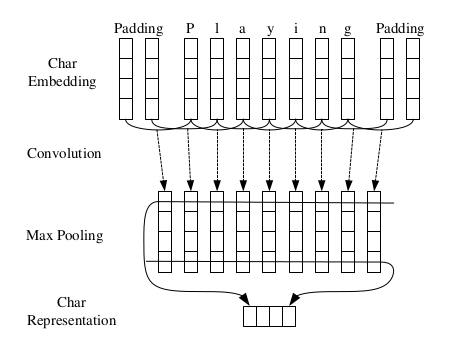
\includegraphics[width=12cm]{Fig_1.png}
	\caption{ La red neuronal de convolución para extraer representaciones de palabras 
	a nivel de carácter. Las flechas discontinuas indican una capa de dropout aplicada antes 
	de que se ingresen los embeddings de caracteres en CNN.}
	\label{F1}
\end{figure}

\newpage

Para esta capa se tomó el tamaño del kernel de convolción como 3, con padding hacia los lados 
no afectando así la dimensión del tamaño de la palabra al salir de la convolución. Como resultado
se obtiene un vector de $W \times 30$ donde 30 es la cantidad de filtros de la capa. Esta salida a su vez
luego es comprimida con un max pooling devolviendo la representación final de la palabra como un
vector de dimensión $1 \times 30$ que será concatenada a la representación de la palabra asociada.

\subsection{LSTM}
	
Las redes neuronales recurrentes (RNN) son una poderosa familia de modelos conexionistas que capturan 
la dinámica del tiempo a través de ciclos en el grafo. Aunque, en teoría, las RNN son capaces de 
capturar dependencias de larga distancia, en la práctica fallan debido a los problemas de 
desaparición/explosión del gradiente (Bengio et al., 1994; Pascanu et al., 2012). Los LSTM 
(Hochreiter y Schmidhuber, 1997) son variantes de los RNN diseñados para hacer frente a estos 
problemas de desaparición de gradientes. Básicamente, una unidad LSTM se compone de tres puertas
multiplicativas que controlan las proporciones de información para olvidar y pasar al siguiente 
paso de tiempo. La Figura 2 muestra la estructura básica de una unidad LSTM.

\begin{figure}
	\centering
	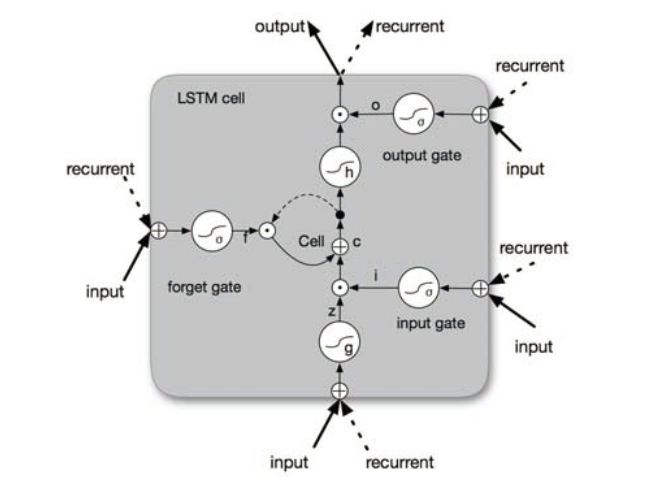
\includegraphics[width=12cm]{Fig_2.png}
	\caption{  Esquema de una unidad LSTM.}
	\label{F2}
\end{figure}

\newpage

Formalmente las fórmulas para actualizar una unidad LSTM en un tiempo t son:

\begin{equation}
i_{t} = \sigma(W_{i} h_{t-1} + U_{i} x_{t} + b_{i})
\end{equation}

\begin{equation}
f_{t} = \sigma(W_{f} h_{t-1} + U_{f} x_{t} + b_{f})
\end{equation}

\begin{equation}
\tilde{c}_{t} = \tanh(W_{c} h_{t-1} + U_{c} x_{t} + b_{c})
\end{equation}

\begin{equation}
c_{t} = f_{t} \odot c_{t-1} + i_{t} \odot \tilde{c}_{t}
\end{equation}

\begin{equation}
o_t = \sigma(W_{o} h_{t-1} + U_{o} x_{t} + b_{o})
\end{equation}

\begin{equation}
h_{t} = o_{t} \odot \tanh( c_{t})
\end{equation}



donde $\sigma$ es la función sigmoidal elemento a elemento y $\odot$ es el producto elemento a elemento. 
$x_{t}$ es el  vector entrada (e.g. embeddings de palabras) en el tiempo $t$, y $h_{t}$ es el 
vector de estado oculto (tambien llamado vector de salida) que guarda toda la información importante 
en (y antes) del tiempo  t. $U_{i}$ , $U_{f}$ , $U_{c}$ , $U_{o}$ denota las matrices de pesos de 
puertas diferentes para la entrada $x_{t}$ , y $W_{i}$ , $W_{f}$ , $ W_{c}$ , $W_{o}$ son las
matrices de pesos para el estado oculto $h_{t}$. $b_{i}$ , $b_{f}$ , $b_{c}$ , $b_{o}$ denotan los 
vectores de bias.

\subsubsection{BLSTM}

Para muchas tareas de etiquetado de secuencias, es beneficioso tener acceso a contextos pasados 
(izquierda) y futuros (derecha). Sin embargo, el estado oculto de LSTM $h_{t}$ toma información 
solo del pasado, sin saber nada sobre el futuro. Una solución elegante cuya eficacia ha sido probada 
por trabajos anteriores (Dyer et al., 2015) es LSTM bidireccional (BLSTM). La idea básica es presentar 
cada secuencia hacia adelante y hacia atrás en dos estados ocultos separados para capturar información 
pasada y futura, respectivamente. Luego, los dos estados ocultos se concatenan para formar la salida 
final.

\subsection{CRF}

Para las tareas de etiquetado de secuencias (o predicción estructurada general), es beneficioso 
considerar las correlaciones entre las etiquetas en los vecindarios y decodificar conjuntamente 
la mejor cadena de etiquetas para una oración de entrada dada. Por ejemplo, en el etiquetado POS, 
es más probable que un adjetivo vaya seguido de un sustantivo que de un verbo, y en NER con anotación 
BIO2 estándar (Tjong Kim Sang y Veenstra, 1999), I-ORG no puede seguir a I-PER. Por lo tanto, 
modelamos la secuencia de etiquetas de forma conjunta utilizando un campo aleatorio condicional 
(CRF) (Lafferty et al., 2001), en lugar de decodificar cada etiqueta de forma independiente. 
Formalmente, usamos $z = \{z_{1}$ ,··· , $z_{n} \}$ para representar una secuencia de entrada 
genérica donde $z_{i}$ es el vector de entrada de la i-ésima palabra. $y = \{y_{1}$ , ··· , $y_n \}$ 
representa una secuencia genérica de etiquetas para $z$. $Y(z)$ denota el conjunto de posibles 
secuencias de etiquetas para $z$. El modelo probabilístico para la secuencia CRF define una 
familia de probabilidad condicional $p(y|z; W, b)$ sobre todas las posibles secuencias de 
etiquetas "y", dado "z" con la siguiente forma:

\begin{equation}
	p(y|z; W, b) =  \frac {\prod_{i=1}^{n} \psi_{i} (y_{i-1}, y_{i} ,z)}
	{\sum_{y' \in Y(z)} \prod_{i=1}^{n} \psi_{i} (y_{i-1}', y_{i}' , z)}
\end{equation}

donde $\psi_{i}(y',y, z) = exp(W_{y',y}^{T} z_{i}+ b_{y',y} )$ son funciones potencia, 
y $W_{y',y}^{T}$ ,$b_{y',y}$  son  el vector de pesos y bias correspondiente al par anotado 
(y' , y), respectivamente. Para el entrenamiento de la CRF , se usa la estimación de la máxima 
verosimilitud condicional. Para un conjunto de entrenamiento ${(z_{i} , y_{i} )}$, el 
logaritmo de la verosimilitud (conocido como la log-verosimilitud) esta dada por:

\begin{equation}
	L(W, b) =\sum_{i}{\log p(y|z; W, b)}
\end{equation}


%TODO REVISAR TODAS LAS FORMULAS DEBEN ESTAR MAL REPRESENTADAS

El entrenamiento de la máxima verosimilitud escoge parámetros tal que la log-verosimilitud 
es maximizada.

Decodificar es buscar la secuencia de la etiqueta $y^*$ con la mayor probabilidad condicional:
\begin{equation}
	y^\ast = argmax_{y\in Y(z)} p(y|z; W, b)
\end{equation}


Para un modelo CRF secuencial (solo se consideran las interacciones entre dos etiquetas sucesivas),
el entrenamiento y la decodificación se pueden resolver de manera eficiente adoptando el algoritmo 
de Viterbi.

\subsection{BLSTM-CNNs-CRF}
	
Finalmente, se construye este modelo de red neuronal alimentando los vectores de salida de BLSTM 
en una capa CRF. La Figura \ref{F3} ilustra la arquitectura de esta red en detalle. Para cada palabra, 
la CNN calcula la representación a nivel de carácter en la Figura \ref{F1} con embeddings de caracteres 
como entradas. Luego, el vector de representación a nivel de carácter se concatena con el vector de 
de palabras para alimentar la red BLSTM. Finalmente, los vectores de salida de BLSTM se 
pasan a la capa CRF para decodificar conjuntamente la mejor secuencia de etiquetas. Como se 
muestra en la Figura \ref{F3}, las capas de exclusión se aplican tanto en los vectores de entrada como 
de salida de BLSTM.

\begin{figure}
	\centering
	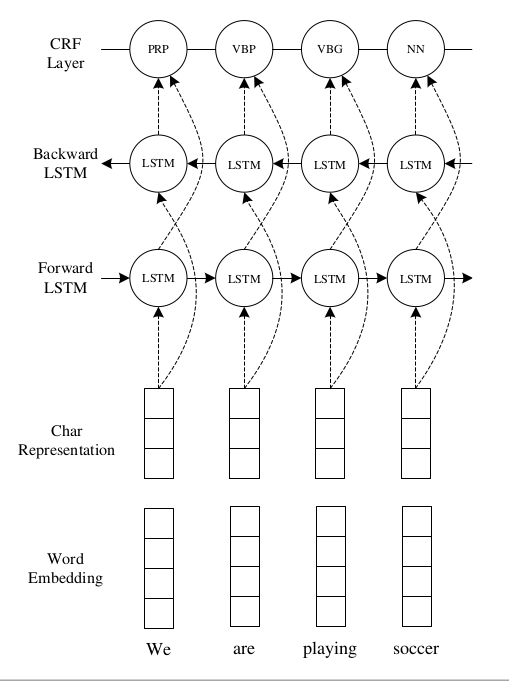
\includegraphics[width=12cm]{Fig_3.png}
	\caption{ La principal arquitectura de la red neuronal.
		La representación de los caracteres de cada palabra
		son computados por la CNN en Figura \ref{F1}. Luego
		la representación es concatenada con el embedding de
		la palabra antes de pasarselo a la red BLSTM. Líneas
		discontinuas indican que capas de dropout son aplicadas
		en la entrada y salida de BLSTM.}
	\label{F3}
\end{figure}


\section{Implementación}

Para la implementación de la red neuronal artificial se utilizó la imagen de docker
\emph{tensorflow/tensorflow:2.9.1-jupyter}. Como su nombre menciona, esta imagen
trae la versión especificada de tensorflow y además está preparada para ser corrida
como un jupyter notebook. Esta imagen no contenía la implementación de CRF por lo que
se creó otra a partir de esta con la biblioteca que lo contenía.

El componente principal del modelo constituyen las capas de este. Para la implementación
se hizo uso de las siguientes \cite{tensorflowDoc} \cite{kerasDoc}:

\begin{itemize}
	\item Vectorizer: Convierte las secuencias en vectores donde cada elemento representa el
	índice de la palabra en un vocabulario.
	\item Embedding: Capa usada para la conversión de vectores de índices en tensores conteniendo
	la representación final del elemento.
	\item Conv1D: Usada para realizar la convolución sobre las secuencias de embeddings de
	caracteres
	\item MaxPooling1D: Usada para calcular la representación final de la palabra basados 
	en los resultados de la convolución
	\item Dropout: Usada para prevenir el overfitting en el conjunto de entrenamiento y
	permitir una correcta generalización del problema
	\item Bidirectional LSTM: Permite que las secuencias se apliquen a la capa LSTM en ambas
	direcciones.
	\item CRF: Calcula una distribución de probabilidad conjunta para clasificar secuencias
	con las etiquetas dadas.
\end{itemize}

\section{Entrenamiento}

\subsection{Corpus Usado}

El corpus usado en el entrenamiento constituye una versión en formato
Conll del corpus Argument Annotated Essays Corpus \cite{corpus}. Este corpus contiene una 
colección de 402 ensayos argumentativos. Además viene con una selección de archivos
para entrenamiento, prueba y validación. Dicho corpus fue segmentado
en oraciones, dando como resultado una división de 5096(70\%), 1452(20\%) y 609(10\%) oraciones para
entrenamiento, prueba y validación respectivamente. 

Para el entrenamiento se hizo preprocesamiento sobre el corpus inicial. Primero se llevaron
las etiquetas de BIO a BIOES, luego se separaron las oraciones de los párrafos y se guardaron
en un archivo con una oración en cada línea. Se hizo algo similar con las anotaciones de la oración.
Además se crearon archivos conteniendo el vocabulario, los caracteres y las etiquetas para futuros
procesamientos.


\subsection{Hiperparámetros y optimización}

La selección de los hiperparámetros del modelo fue basada en las sugerencias dadas en
\cite{paper}.

\begin{itemize}
	\item Droput rate: 0.5
	\item Filtros: 30
	\item Tamaño de kernel: 3
	\item Cantidad unidades en LSTM: 200  
\end{itemize}

\subsection{Duración}

El modelo se corrió durante 25 épocas en un i5-6200U CPU @ 2.30GHz. Cada época
duró aproximadamente 2 minutos, con un total de 50 minutos de entrenamiento.

\section{Evaluación}

Para la evaluación se tomaron las medidas de accuracy y de la función de pérdida y se
crearon gráficas con los valores para ser examinados. Para tener más referencias se
crearon modelos alternativos al propuesto. Entre estos se encuentran variantes del
modelo sin la capa de embeddigns de caracteres y variantes que conectan a la salida
de la capa BLSTM una red densa con la capa CRF. Las variantes tendrán las siguientes
signaturas, CNN si tiene la capa de convolción de los caracteres y DL si tiene la capa
densa.

\subsection{Resultados}

\begin{table}
	\centering
	\caption{Resultados.}\label{results}
	\begin{tabular}{|l|l|l|}
	\hline
		Arq. &  Accuracy & Loss \\
	\hline
		CNN-BLSTM-DL-CRF & 0.9097 & 0.6028 \\
		CNN-BLSTM-CRF 	  & 0.9080 & 0.5299 \\
		BLSTM-DL-CRF 	  & 0.8868 & 0.7424 \\
		BLSTM-CRF 		  & 0.8923 & 0.8415 \\
	\hline
	\end{tabular}
\end{table}

Como se observa en la Tabla \ref{results} la arquitectura con la capa de convolución
presenta mejor desempeño en todos los aspectos. Las arquitecturas basadas en CNN 
contienen un accuracy semejante, aunque su diferencia en la pérdida es un poco más
grande.

\begin{figure}
	\centering
	\includegraphics[width=12cm]{model_cnn_BiLSTM_crf_acc.png}
	\caption{Accuracy durante entrenamiento CNN-BLSTM-CRF}
	\label{acc_fig}
\end{figure}

\begin{figure}
	\centering
	\includegraphics[width=12cm]{model_cnn_BiLSTM_crf_loss.png}
	\caption{Pérdida durante entrenamiento CNN-BLSTM-CRF}
	\label{loss_fig}
\end{figure}

\section{Conclusiones}

El modelo propuesto resuelve el problema con una accuracy aproximada del 90\%. Este
resultado satisface las métricas deseadas del problema de segmentación de componentes
argumentativas. 

\begin{thebibliography}{8}

\bibitem{tensorflowDoc}
TensorFlow Documentation \url{https://www.tensorflow.org/api_docs} 

\bibitem{kerasDoc}
Keras Documentation, \url{https://faroit.com/keras-docs/1.2.0/}

\bibitem{paper}
Ma, Xuezhe and Hovy, Eduard:
End-to-end sequence labeling via bi-directional lstm-cnns-crf:
arXiv preprint arXiv:1603.01354 . 2016 

\bibitem{corpus}
Christian Stab and Iryna Gurevych. 2016. Parsing Argumentation Structure in 
Persuasive Essays. arXiv preprint

\end{thebibliography}

\end{document}
